\section{Springer Theory}
\label{chapter_springer}

This chapter provides an overview of Springer theory. Most of the statements and proofs come from \cite{chriss1997representation}, where a thorough treatment on the topic is included.

\subsection{Semisimple Lie Groups and Lie Algebras}

Let $G$ be a complex semisimple connected Lie group with a Lie algebra $\lie{g}$. The adjoint action of $G$ on $\lie{g}$ will be denoted by $g \cdot x$ for $g \in G$ and $x \in \lie{g}$. Fix a Borel subgroup $B \subseteq G$. Let $U \subseteq B$ be the unipotent radical and $T \subseteq B$ be a maximal torus. Denote by $\lie{b}$, $\lie{n}$ and $\lie{h}$ the Lie algebra of $B$, $U$ and $T$ respectively. The Killing form is a canonical $G$-invariant non-degenerate symmetric bilinear form on $\lie{g}$, which allows us to identify $\lie{g}$ with its dual. This carries the Poisson structure on $\lie{g}^*$ to $\lie{g}$, where the symplectic leaves are precisely the adjoint orbits.

The $T$-action on $\lie{g}$ splits into weight spaces. Let
\begin{enumerate}
    \item $\Phi \subseteq \lie{h}_\mathbb{Z}^*$ denote the set of roots, i.e. the non-trivial $T$-weights on $\lie{g}$,
    \item $\Phi^+ \subseteq \Phi$ denote the set of positive roots, i.e. the non-trivial $T$-weights on $\lie{b}$,
    \item $\Phi^- = \Phi \setminus \Phi^+$ denote the set of negative roots,
    \item $\Delta \subseteq \Phi^+$ denote the set of simple roots, i.e. the positive roots that cannot be written as a positive linear combination of other positive roots.
\end{enumerate}
This gives the weight decomposition $\lie{g} \cong \lie{h} \oplus \bigoplus_{\alpha \in \Phi} \lie{g}_\alpha$, where each $\lie{g}_\alpha$ is one-dimensional. Write $\lie{n}^- = \bigoplus_{\alpha \in \Phi^-} \lie{g}_\alpha$, giving us the triangular decomposition $\lie{g} = \lie{n}^- \oplus \lie{h} \oplus \lie{n}$.

The Weyl group of $G$ is a finite group defined by $W = N_G(T)/T$. The conjugation action of $W$ on $T$ descends to an action on $\lie{h}$ and $\lie{h}^*$ fixing the roots. The connected components in $\lie{h}_\mathbb{R} \setminus \bigcup_{\alpha \in \Phi} \alpha^\perp$ are called the Weyl chambers. The Weyl group $W$ act on the set of Weyl chambers simply transitively. The chamber that pair all positive roots positively is called the dominant chamber. We will abuse the notation to denote by $w \in W$ an arbitrary choice of representative $w \in N_G(T)$.

\begin{definition}[def:]{}
    An element $x \in \lie{g}$ is
    \begin{itemize}
        \item \vocab{regular} if $\dim Z_{\lie{g}}(x) = \operatorname{rk} \lie{g}$, where $Z_{\lie{g}}(x)$ is the centralizer of $x$ in $\lie{g}$ and $\operatorname{rk} \lie{g}$ is the dimension of $\lie{h}$,
        \item \vocab{semisimple} if $\operatorname{ad} x : \lie{g} \to \lie{g}$ is diagonalizable,
        \item \vocab{nilpotent} if $\operatorname{ad} x : \lie{g} \to \lie{g}$ is nilpotent.
    \end{itemize}
    Write $\lie{g}^{\mathrm{reg}}$ for the set of regular elements, $\lie{g}^{\mathrm{sr}}$ for the set of semisimple regular elements and $\nilcone$ for the set of nilpotent elements.
\end{definition}

Let $\borel$ be the variety of Borel subgroups of $G$ (or equivalently, of Borel subalgebras of $\lie{g}$). It carries a left $G$-action by conjugation. The $G$-stabilizer of a point in $\borel$ is the precisely the Borel subgroup represented by that point.
\begin{lemma}[lem:]{}
    $\borel \cong G/B$.
    \begin{proof}
        Since all Borel subgroups are conjugate to each other, the $G$-action on $\borel$ is transitive. The stabilizer of $B \in \borel$ is $B$ itself. Thus, $G/B \cong \borel$ with $gB \in G/B \mapsto gBg^{-1} \in \borel$ is an isomorphism.
    \end{proof}
\end{lemma}
It follows that $\dim \borel = \dim G - \dim B = \frac{1}{2}(\dim \lie{g} - \operatorname{rk} \lie{g})$.

\begin{lemma}[lem:bruhat_decomposition]{Bruhat decomposition}
    $W \cong \borel^T \cong B\backslash G/B \cong B \backslash \borel \cong G \backslash (\borel \times \borel)$.
    \begin{proof}
        The isomorphisms is given by
        \begin{equation*}
            w \in W \mapsto wB \in \borel \mapsto B \cdot w \cdot B \in B\backslash G/B \mapsto B \cdot wB \in B \backslash \borel \mapsto G \cdot (B, wB) \in G \backslash (\borel \times \borel),
        \end{equation*}
        where we identified $\borel \cong G/B$ and chose a representative for each $w \in W$ implicitly.

        We first compute the $T$-fixed points of $\borel$. Note that $\borel^T$ is precisely the set of Borel subgroups containing $T$. Then, $N_G(T)$ acts on this set by conjugation. We claim that is action is transitive with stabilizer $T$. Let $gBg^{-1} \in \borel^T$. Then, $g^{-1}Tg \subseteq B$. Thus, $g^{-1}Tg = bTb^{-1}$ for some $b \in B$, implying that $gb \in N_G(T)$. Hence, $gBg^{-1} = gbB(gb)^{-1}$, showing transitivity. On the other hand, the stabilizer at $B \in \borel^T$ is given $N_G(T) \cap B = N_B(T) = T$.
        
        Define $\schubert_w$ to be the $B$-orbit of the $T$-fixed point $wB \in G/B$. Since the $G$-stabilizer at $wB$ is $wBw^{-1}$, we have $B$-equivariant isomorphisms
        \begin{equation*}
            \schubert_w \cong B / (B \cap wBw^{-1}) \cong U / (U \cap wUw^{-1}) \cong \lie{n} / (\lie{n} \cap w \cdot \lie{n}) \cong \lie{n} \cap w \cdot \lie{n}^-.
        \end{equation*}
        It follows that every $\schubert_w$ contains a unique $T$-fixed point $wB$, hence they are all distinct. To show that every point in $G/B$ is contained in some $\schubert_w$, fix $h \in \lie{h}_\mathbb{Z}$ in (the interior of) the dominant chamber (which is automatically regular). Then, the fixed points of the corresponding one-parameter subgroup action on $G/B$ are precisely the $T$-fixed points. Define
        \begin{equation*}
            \schubert_w' = \left\{ gB \in G/B \mid \lim_{t \to 0} t \cdot gB = wB \right\}.
        \end{equation*}
        Since $G/B$ is projective, the limit above always exists, so $G/B = \bigsqcup_{w \in W} \schubert_w'$. We claim that $\schubert_w' = \schubert_w$. Since $\lim_{t \to 0} tut^{-1} = 1$ for all $u \in U$, we have
        \begin{equation*}
            \lim_{t \to 0} t \cdot uwB = \lim_{t \to 0} tut^{-1} \cdot wB = wB.
        \end{equation*}
        Hence, $\schubert_w = U \cdot wB \subseteq \schubert_w'$. Note that $T_{wB}\schubert_w' = T_{wB} \schubert_w \cong \lie{n} \cap w \cdot \lie{n}^-$, so $\schubert_w$ is closed in $\schubert_w'$. On the other hand, any orbit of a unipotent group is closed. Since $\schubert_w'$ is connected, we have $\schubert_w = \schubert_w'$.
    \end{proof}
\end{lemma}

The double cosets $\{BwB\}_{w \in W}$ in $G$ are called the \vocab{Bruhat cells}, and the $B$-orbits $\{\schubert_w\}_{w \in W}$ in $G/B$ are called the \vocab{Schubert cells}. We have
\begin{equation*}
    \overline{BwB} = \bigsqcup_{w' \leq w} Bw'B \quad \text{and} \quad \overline{\schubert_w} = \bigsqcup_{w' \leq w} \schubert_{w'}
\end{equation*}
for all $w \in W$, where $\leq$ is the Bruhat order on $W$.

\subsection{Bruhat Order}

\begin{definition}[def:]{}
    A \vocab{Coxeter System} is a finite set $S$ together with a map
    $m:S\times S\rightarrow \mathbb{Z}_{\geq 1}\cup \CB{+\infty }$ such that $m(s,s')=m(s',s)$ for all $s,s'\in S$ and $m(s,s')=1$ if and only if $s=s'$. The associated \vocab{Coxeter group} is the group $W$ generated by $S$ with the relations $(ss')^{m(s,s')}=1$ unless $m(s,s')=+\infty$.
\end{definition}

It is known that Weyl groups of semi-simple Lie Groups are Coxeter groups.
We will demostrate the example of type A Weyl groups as Coxeter groups.

\begin{example}[exp:]{}
    Let $S=\CB{s_1,\dots ,s_{n-1}}$ and define
    \[
        m(s_i,s_j)
        =
        \begin{cases}
            1 & i=j,\\
            2 & |i-j|\geq 2,\\
            3 & |i-j|=1.
        \end{cases}
    \]
    $m(s_i,s_j)=2$ means $s_i$ and $s_j$ commutes, and $m(s_i,s_{i+1})=3$ gives the braid relations $s_is_{i+1}s_i=s_{i+1}s_is_{i+1}$.
    Hence the assoicated Coxeter group is $W=S_n$.
\end{example}

Let $W$ be a Coxeter group.
Any $w\in W$ can be written as $w=s_1s_2\dots s_k$, where $s_i\in S$, called the \vocab{word representative}. We call a word \vocab{reduced} if it has the minimal length among all word representatives. And the length $l(w)$ of $w$ is defined as the length of any reduced word.

The \vocab{Bruhat order} on the set of elements in $W$ is a partial order. Let $w=s_1s_2\dots s_{l(w)}$ be a reduced word. We say $v\leq w$ in the bruhat order if and only if there exist indices $1\leq i_1<\cdots <i_k\leq l(w)$ such that $v=s_{i_1}s_{i_2}\dots s_{i_k}$.

\begin{example}[exp:]{}
\end{example}

In general, it is difficult to determine the bruhat order.
For type $A$ Weyl groups, let $w\in S_n$ and $i,j\in \CB{1,\dots ,n}$. Define
\[
    w[i,j]=\#\CB{h\leq i\mid w(h)>j}.
\]
We have the following Tableau Criterion to check the Bruhat order.

\begin{theorem}[thm:]{}
    For $v,w\in W$. The following are equivalent:
    \begin{enumerate}
        \item $v\leq w$ in the Bruhat order.
        \item For all $i,j\in \CB{1,\dots ,n}$, $v[i,j]\leq w[i,j]$.
        \item For all $i\in \CB{2,\dots ,n}$ and $j\in \CB{1,\dots ,n-1}$ such that
            \[
                v^{-1}(i)>v^{-1}(i+1)\textnormal{ and }v(j)>v(j+1),
            \]
            $v[i,j]\leq w[i,j]$.
    \end{enumerate}
\end{theorem}

\begin{example}[exp:]{}
\end{example}


% This algebra can be regarded as a \( G \)-module through the adjoint action. Let \( B \) be a Borel subgroup, defined as a maximal solvable subgroup of \( G \). Additionally, let \( T \) be a maximal torus contained within \( B \), and let \( U \) denote the unipotent radical of \( B \), such that \( B = T \cdot U \). Note that \( B \) is connected. The corresponding Lie algebras of \( B, T, U \) are represented by \( \mathfrak{b}, \mathfrak{h}, \mathfrak{n} \), respectively, where \( \mathfrak{b} = \mathfrak{h} \oplus \mathfrak{n} \) and \( \mathfrak{n} = [\mathfrak{b}, \mathfrak{b}] \). The subalgebra \( \mathfrak{h} \) is identified as a Cartan subalgebra of \( \mathfrak{g} \), and its dimension, denoted \( \dim \mathfrak{h} = \text{rk} \mathfrak{g} \), is referred to as the rank of \( \mathfrak{g} \).

% Denote by $Z_G(x)$ and $Z_\mathfrak{g}(x)$ the centralizer of $ x \in \mathfrak{g} $ in $ G $ and $ \mathfrak{g} $ respectively.
% For any element $ x \in \mathfrak{g} $, we have
% \[
% \dim Z_\mathfrak{g}(x) \geq \text{rk} \mathfrak{g}.
% \]
% We call an element $x\in \mathfrak{g}$ \vocab{regular} if the equality holds, i.e. $ \dim Z_\mathfrak{g}(x) = \text{rk} \mathfrak{g} $.
% We call an element $x\in \mathfrak{g}$ \vocab{semisimple}  if $ \text{ad} \, x : \mathfrak{g} \to \mathfrak{g} $ is diagonalizable, and \vocab{nilpotent} if $\text{ad}\ x$ is nilpotent.
% Denote by $ \mathfrak{g}^{sr} $ the set of regular semisimple elements in $ \mathfrak{g} $.
% The Jordan decomposition theorem says that for any element $ x \in \mathfrak{g} $, we can write $ x = s + n $, where $ s $ is semisimple, $ n $ is nilpotent, and they commute, i.e., $ [s, n] = 0 $. And hence $ s $ and $ n $ commute with $ x $.

% Pick a Borel subgroup $ B \subset G $ and a maximal torus $ T \subset B $. And define the Weyl group $ W_T = N_G(T) / T $ with respect to $T$, where $ N_G(T) $ is the normalizer of $ T $ in $ G $. There are various geometric interpretations of $ W_T $, allowing us to form a notion of abstract Weyl group $W$.

% One clearly have the map $ W_T \to B \backslash G / B $, sending $ w \in W_T $ to the double coset $ B w B $, where $ w $ is a representative of $ w $ in $ N(T) $.
% Define $ \mathfrak{B} $ the set of all Borel subgroups in $G$. 
% There is an $G$-equivariant isomorphism of algebraic varieties $G/B\rightarrow \mathfrak{B}$, $gB \mapsto gB g^{-1}$. And hence a bijection $ B \backslash G / B \to \{B\text{-orbits on } \mathfrak{B}\} $ sending a double coset $ B g B $ to the $ B $-orbit of the right coset $ g B / B \in G/B $.

% We further have a map $ \{B\text{-orbits on } \mathfrak{B}\} \to \{G\text{-diagonal orbits on } \mathfrak{B} \times \mathfrak{B}\} $ sending the $ B $-orbit of a point $ b \in \mathfrak{B} $ to the $ G $-diagonal orbit of the point $ (b_0, b) \in \mathfrak{B} \times \mathfrak{B} $.
% %It is noteworthy that $ \{b_0\} $ represents the sole one-point $ B $-orbit in $ \mathfrak{B} $, and this mapping assigns it to the diagonal in $ B \times \mathfrak{B} $, which forms the $ G $-orbit in $ \mathfrak{B} \times \mathfrak{B} $ of minimal dimension.

% We have the following theorem:

% \begin{theorem}[thm:]{}
%   The mapss are bijections:
% \[
% W_T \to B \backslash G / B \to \{B\text{-orbits on } \mathfrak{B}\} \to \{G\text{-diagonal orbits on } \mathfrak{B} \times \mathfrak{B}\}.
% \]
% \end{theorem}

% We should note that there is also a bijection of $T$-fixed points in $\mathfrak{B}$ with $W_T$.

% $(B_1,B_2)\in \mathfrak{B}\times \mathfrak{B}/\triangle G$ is said to be in relative position $w$ if its index in $W_T$ is $w$.

% Fixing a Borel $B\subseteq G$, $\mathfrak{B}\simeq G/B$ is called the \vocab{flag variety}.

% \begin{theorem}[thm:]{}
%   $\mathfrak{B}$ is a smooth projective variety. Moreover, there exist an explicit embedding $\iota:\mathfrak{B}\hookrightarrow P(V)$, where $V$ is a finite dimensional irreducible $G$-representation.
% \end{theorem}

\subsection{Springer Resolution}

Define
\begin{align*}
    \tilde{\lie{g}} &= \{ (\lie{b}', x) \mid \lie{b}' \in \borel, x \in \lie{b}' \} \cong G \times_B \lie{b}, \\
    \tilde{\nilcone} &= \{ (\lie{b}', x) \mid \lie{b}' \in \borel, x \in \lie{b}' \cap \nilcone \} \cong G \times_B \lie{n}.
\end{align*}
There are evident maps $\mu : \tilde{\lie{g}} \to \lie{g}$ and $\mu : \tilde{\nilcone} \to \nilcone$.

\begin{lemma}[lem:]{}
    The projection $\tilde{\nilcone} \to \borel$ given by $(\lie{b}', x) \mapsto \lie{b}'$ is isomorphic to the cotangent bundle of $\borel$. 
    \begin{proof}
        Using the identification $\borel \cong G/B$, note that the cotangent space of $gB \in G/B$ is given by $(g \cdot \lie{b})^\perp \cong g \cdot \lie{n}$, where the isomorphism is given by the Killing form. On the other hand, the fiber of the map $\tilde{\nilcone} \to \borel$ at $gB$ is also given by $g \cdot \lie{b} \cap \nilcone = g \cdot \lie{n}$.
    \end{proof}
\end{lemma}
For any $\lie{b}' \in \borel$, there is a canonical isomorphism $\lie{b}'/[\lie{b}', \lie{b}'] \cong \lie{h}$. Explicitly, if $\lie{b}' = g \cdot \lie{b}$, this map sends $x + [\lie{b}', \lie{b}'] \in \lie{b}'/[\lie{b}', \lie{b}']$ to $[g^{-1} \cdot x]_{\lie{h}} \in \lie{h}$, where $[-]_{\lie{h}} : \lie{g} \to \lie{h}$ is the projection onto the $\lie{h}$ factor along the triangular decomposition $\lie{g} \cong \lie{n} \oplus \lie{h} \oplus \lie{n}^-$. This gives a map $\nu : \tilde{\lie{g}} \to \lie{h}$, which sends $(\lie{b}', x) \in \tilde{\lie{g}}$ to the image of $x$ along $\lie{b}' \to \lie{b}'/[\lie{b}', \lie{b}'] \cong \lie{h}$. Using the identification $\tilde{\lie{g}} \cong G \times_B \lie{b}$, we have $\nu^{-1}(h) = G \times_B (h + \lie{n})$. In particular, $\nu^{-1}(h) = \tilde{\nilcone}$.

Denote $\tilde{\lie{g}}^{\mathrm{sr}} = \mu^{-1}(\lie{g}^{\mathrm{sr}}) \subseteq \tilde{\lie{g}}$, the restriction of $\mu : \tilde{\lie{g}} \to \lie{g}$ to semisimple regular elements. Equivalently, $\tilde{\lie{g}}^{\mathrm{sr}} = \nu^{-1}(\lie{h}^{\mathrm{reg}})$.
\begin{proposition}[prop:W_bun]{}
    The restriction $\tilde{\lie{g}}^{\mathrm{sr}} \to \lie{g}^{\mathrm{sr}}$ is a principal $W$-bundle.
    \begin{proof}
        Note that the $W$-action on $\lie{h}^{\mathrm{reg}}$ is free, giving a principle $W$-bundle $\lie{h}^{\mathrm{reg}} \to \lie{h}^{\mathrm{reg}}/W$. We claim that
        \begin{equation*}
            \begin{tikzcd}
                \tilde{\lie{g}}^{\mathrm{sr}} \arrow[r, "\nu"] \arrow[d, "\mu"'] & \lie{h}^{\mathrm{reg}} \arrow[d] \\
                \lie{g}^{\mathrm{sr}} \arrow[r] & \lie{h}^{\mathrm{reg}}/W
            \end{tikzcd}
        \end{equation*}
        is a pullback square, where the bottom map is the composite of the projection $\lie{g} \to \lie{h}$ along the triangular decomposition with the quotient map. Let $x \in \lie{g}^{\mathrm{sr}}$. Then, $Z_\lie{g}(x)$ is a Cartan subalgebra. Thus, any Borel subalgebra containing $x$ must contain $Z_\lie{g}(x)$. By \Cref{lem:bruhat_decomposition}, the set of Borel subalgebras containing a fixed Cartan subalgebras has a free and transitive $W$-action. By definition, $\nu$ is equivariant under this action. The claim follows.
    \end{proof}
\end{proposition}

\subsection{Steinberg Variety}
\label{sec:steinberg_variety}

Define $\steinberg_{\lie{g}} = \tilde{\lie{g}} \times_{\lie{g}} \tilde{\lie{g}}$ and $\steinberg = \tilde{\nilcone} \times_{\nilcone} \tilde{\nilcone}$. Note that
\begin{align*}
    \steinberg_\lie{g} &\cong \{ (gB, g'B, x) \mid x \in g \cdot \lie{b} \cap g' \cdot \lie{b} \}, \\
    \steinberg &\cong \{ (gB, g'B, x) \mid x \in g \cdot \lie{n} \cap g' \cdot \lie{n} \}.
\end{align*}
There is an evident map $\steinberg \to \nilcone$ and an inclusion $\steinberg \hookrightarrow \tilde{\nilcone} \times \tilde{\nilcone} \cong T^*(\borel \times \borel)$\footnote{The isomorphism $T^*\borel \times T^*\borel \to T^*(\borel \times \borel)$ is given by $(gB, x, g'B, x') \mapsto (gB, g'B, x, -x')$.}.

\begin{lemma}[lem:irr_steinberg]{}
    The image of $\steinberg \hookrightarrow T^*(\borel \times \borel)$ is the union of the conormal bundles of the $G$-orbits of $\borel \times \borel$.
    \begin{proof}
        The $G$-stabilizer of a point $(gB, g'B) \in \borel \times \borel$ is given by $gBg^{-1} \cap g'B(g')^{-1}$. It follows that the conormal fiber of its $G$-orbit at this point is the annihilator of the Lie algebra of this stabilizer, i.e. $g \cdot \lie{n} \cap g' \cdot \lie{n}$.
    \end{proof}
\end{lemma}

By \Cref{lem:bruhat_decomposition}, the $G$-orbits of $\borel \times \borel$ are indexed by $W$. Denote by $\steinberg_w$ the conormal bundle of the $G$-orbit corresponding to $w \in W$. We thus have $\steinberg = \bigsqcup_{w \in W} \steinberg_w$. Since each $\steinberg_w$ is irreducible and of the same dimension, $\{\overline{\steinberg_w}\}_{w \in W}$ is the set of irreducible components of $\steinberg$.

\begin{theorem}[thm:orb_var_lag]{}
    The irreducible components of $\nilorbit \cap \lie{n}$ are Lagrangian subvarieties of $\nilorbit$.
\end{theorem}

For a $G$-orbit $\nilorbit$ in $\nilcone$, write $\tilde{\nilorbit} = \mu^{-1}(\nilorbit) \subseteq \tilde{\nilcone}$ and $\steinberg_\nilorbit = \tilde{\nilorbit} \times_{\nilorbit} \tilde{\nilorbit} \subseteq \steinberg$. Note that $\mu : \tilde{\nilorbit} \to \nilorbit$ gives $\tilde{\nilorbit} \cong G \times_{Z_G(x)} \borel_x$ for any choice of $x \in \nilorbit$, while $ \pi : \tilde{\nilorbit} \to \borel$ gives $\tilde{\nilorbit} \cong G \times_B (\nilorbit \cap \lie{n})$. By \Cref{thm:orb_var_lag}, $\nilorbit \cap \lie{n}$ has pure dimension $\frac{1}{2} \dim \nilorbit$. It follows that
\begin{enumerate}
    \item $\tilde{\nilorbit}$ has pure dimension $\dim \borel + \frac{1}{2} \dim \nilorbit$,
    \item $\borel_x$ has pure dimension $\dim \borel - \frac{1}{2} \dim \nilorbit$ for any $x \in \nilorbit$, and
    \item $\steinberg_\nilorbit$ has pure dimension $2\dim \borel$.
\end{enumerate}
But by \Cref{lem:irr_steinberg}, the irreducible components of $\steinberg$ all have dimension $2\dim \borel$. Thus, the set of closures of the irreducible components of $\steinberg_\nilorbit$ over all nilpotent orbits $\nilorbit$ coincides with the set $\{\overline{\steinberg_w}\}_{w \in W}$ of irreducible components of $\steinberg$. These are summarized as follows.

\begin{corollary}[cor:irr_comp]{}
    We have the following isomorphisms, where $\mathrm{Irr}(X)$ denotes the set of irreducible components of $X$.
    \begin{enumerate}
        \item $\mathrm{Irr}(\tilde{\nilorbit}) \cong \pi_0(Z_G(x))\backslash\mathrm{Irr}(\borel_x) \cong \mathrm{Irr}(\nilorbit \cap \lie{n})$ for any $x \in \nilorbit$.
        \item $\mathrm{Irr}(\steinberg_\nilorbit) \cong \pi_0(Z_G(x))\backslash(\mathrm{Irr}(\borel_x) \times \mathrm{Irr}(\borel_x))$ for any $x \in \nilorbit$.
        \item $\mathrm{Irr}(\steinberg) \cong \bigsqcup_{\nilorbit \in G \backslash \nilcone} \pi_0(Z_G(x_\nilorbit))\backslash(\mathrm{Irr}(\borel_{x_\nilorbit}) \times \mathrm{Irr}(\borel_{x_\nilorbit})) \cong W$, where $x_\nilorbit$ is an arbitrary choice of element in $\nilorbit$.
    \end{enumerate}
\end{corollary}

Recall from \Cref{sec:steinberg} that we have a convolution algebra structure on $\HBM_{4d-\bullet}(\steinberg)$ with action on $\HBM_\bullet(\borel_x)$ for all $x \in \nilcone$, where $d = \dim_\mathbb{C} \borel$. To understand this algebra, we need to study $\steinberg_\lie{g}$.

There is an evident map $\steinberg_\lie{g} \to \borel \times \borel$. Recall by \Cref{lem:bruhat_decomposition} that the orbits of $\borel \times \borel$ are given by $\{ G \cdot (B, wB) \cong G/(B \cap wBw^{-1}) \}_{w \in W}$. Denote by $\Lambda_w$ the preimage of the orbit indexed by $w \in W$, i.e.
\begin{equation*}
    \Lambda_w \cong \{ (gB, g'B, x) \mid x \in g \cdot \lie{b} \cap g' \cdot \lie{b}, g^{-1}g' \in BwB \} \cong G \times_{B \cap wBw^{-1}} (\lie{b} \cap w \cdot \lie{b}).
\end{equation*}
This isomorphism sends $[g, x]$ in the right to $(gB, gwB, g \cdot x)$ in the middle. It follows that $\Lambda_w$ is irreducible of dimension $\dim G$ for all $w \in W$. Thus, the irreducible components of $\steinberg_\lie{g}$ is given by $\{ \overline{\Lambda_w} \}_{w \in W}$.

On the other hand, recall that we have $\nu : \tilde{\lie{g}} \to \lie{h}$. This gives two projections $\nu_1, \nu_2 : \steinberg_\lie{g} \to \lie{h}$. On $\Lambda_w$, we have
\begin{align*}
    \nu_1(gB, gwB, x) &= \nu(gB, x) = [g^{-1} \cdot x]_\lie{h}, \\
    \nu_2(gB, gwB, x) &= \nu(gwB, x) = [w^{-1}g^{-1} \cdot x]_\lie{h} = w^{-1} \cdot [g^{-1} \cdot x]_\lie{h}.
\end{align*}
Thus, $\nu_2|_{\Lambda_w} = w^{-1} \cdot \nu_1|_{\Lambda_w}$. For any $S \subseteq \lie{h}$, note that
\begin{equation*}
    \nu_1^{-1}(S) \cap \Lambda_w = \nu_2^{-1}(w^{-1} \cdot S) \cap \Lambda_w \cong G \times_{B \cap wBw^{-1}} (S + \lie{n} \cap w \cdot \lie{n}).
\end{equation*}

Let $S \subseteq \lie{h}$ and $w \in W$. The action by $w^{-1}$ restricts to $S \to w^{-1} \cdot S$, which induces a graph $\{ (h, w^{-1} \cdot h) \mid h \in S \}$ in $\lie{h} \times \lie{h}$. Denote by $\Lambda_w^S$ the preimage of this set along $(\nu_1, \nu_2) : \steinberg_\lie{g} \to \lie{h} \times \lie{h}$. Explicitly,
\begin{equation*}
    \Lambda_w^S = \{ (gB, g'B, x) \mid x \in g \cdot \lie{b} \cap g' \cdot \lie{b}, \nu(gB, x) \in S, \nu(g'B, x) = w^{-1} \cdot \nu(gB, x) \}.
\end{equation*}
This is clearly a closed subset in $\steinberg_\lie{g}$. When $S = \{ 0 \}$, we have $\Lambda_w^S = \steinberg$ for all $w \in W$. For $S \subseteq \lie{h}^\mathrm{reg}$, we have the following commutative square.
\begin{equation*}
    \begin{tikzcd}
        \nu^{-1}(S) \arrow[r, "{w^{-1}}", "\sim"'] \arrow[d, "\nu"'] & \nu^{-1}(w^{-1} \cdot S) \arrow[d, "\nu"] \\
        S \arrow[r, "{w^{-1}}"', "\sim"] & w^{-1} \cdot S
    \end{tikzcd}
\end{equation*}
It follows that $\Lambda_w^S$ is the graph of the top arrow, which also equals the set $\nu_1^{-1}(S) \cap \Lambda_w$ analyzed above. Applying the convolution construction in \Cref{sec:steinberg} to $M_1 = \nu^{-1}(S)$, $M_2 = \nu^{-1}(w^{-1} \cdot S)$, $M_3 = \nu^{-1}((w')^{-1}w^{-1} \cdot S)$, $Z_{12} = \Lambda_w^S$, $Z_{23} = \Lambda_{w'}^{w^{-1} \cdot S}$ and $Z_{13} = \Lambda_{ww'}^S$, we obtain a convolution product
\begin{equation*}
    {*} : \HBM_\bullet(\Lambda_w^S) \otimes \HBM_\bullet(\Lambda_{w'}^{w^{-1} \cdot S}) \to \HBM_\bullet(\Lambda_{ww'}^S).
\end{equation*}

\begin{theorem}[thm:]{}
    There is an algebra isomorphism $\HBMtop(\steinberg) \cong \mathbb{C}[W]$.
    \begin{proof}
        Fix a real two-dimensional subspace $\lie{l} \subseteq \lie{h}$ such that $\lie{l}^* = \lie{l} \setminus \{ 0 \} \subseteq \lie{h}^\mathrm{reg}$. Write $[\Lambda_w^0]$ for the image of the fundamental class $[\Lambda_w^{\lie{l}^*}]$ along the specialization map
        \begin{equation*}
            \HBMtop(\Lambda_w^{\lie{l}^*}) \to \HBMtop(\Lambda_w^{\{0\}}) = \HBMtop(\steinberg).
        \end{equation*}
        We claim that the map $\mathbb{C}[W] \to \HBMtop(\steinberg)$ sending $w$ to $[\Lambda_w^0]$ gives an algebra isomorphism.
        
        To show that this is an isomorphism of vector spaces, note that the fundamental classes of the irreducible components $\{[\overline{\steinberg_w}]\}_{w \in W}$ forms a basis of $\HBMtop(\Lambda_w^{\steinberg})$. Since $[\Lambda_w^{\lie{l}^*}]$ is supported in the irreducible component $\overline{\Lambda_w}$ in $\steinberg_\lie{g}$, $[\Lambda_w^0]$ is supported in the irreducible component $\overline{\Lambda_w} \cap \steinberg \subseteq \bigcup_{w' \leq w} \overline{\steinberg_{w'}}$ of $\steinberg$. Thus, $[\Lambda_w^0]$ is a linear combination of $\{[\overline{\steinberg_{w'}}]\}_{w' \leq w}$. On the other hand, we have
        \begin{equation*}
            \Lambda_w^{\lie{l}^*} = G \times_{B \cap wBw^{-1}} (\lie{l}^* + \lie{n} \cap w \cdot \lie{n}) \xrightarrow{\text{limits to}} G \times_{B \cap wBw^{-1}} (\lie{n} \cap w \cdot \lie{n}) = \steinberg_w
        \end{equation*}
        on the open part. Thus, the coefficient of $[\overline{\steinberg_w}]$ in the linear combination is $1$. This shows the linear independency of the classes $\{[\Lambda_w^0]\}_{w \in W}$.
        
        For the algebra structure, set $S = \lie{l}^*$ in the argument above the theorem. We have a convolution product
        \begin{equation*}
            {*} : \HBM_\bullet(\Lambda_w^{\lie{l}^*}) \otimes \HBM_\bullet(\Lambda_{w'}^{w^{-1} \cdot {\lie{l}^*}}) \to \HBM_\bullet(\Lambda_{ww'}^{\lie{l}^*}).
        \end{equation*}
        In fact, the product preserves the fundamental classes, i.e. $[\Lambda_w^{\lie{l}^*}] * [\Lambda_{w'}^{w^{-1} \cdot {\lie{l}^*}}] = [\Lambda_{ww'}^{\lie{l}^*}]$. Taking specialization, we obtain the equality $[\Lambda_w^0] * [\Lambda_{w'}^0] = [\Lambda_{ww'}^0]$.
    \end{proof}
\end{theorem}

We now analyze how $\HBMtop(\steinberg) \cong \mathbb{C}[W]$ acts on $\HBM_\bullet(\borel_x)$ for $x \in \nilcone$. Note that \Cref{sec:steinberg} showed that $\HBM_\bullet(\borel_x)$ has a $\HBMtop(\steinberg)$-bimodule structure, related by the anti-involution on $\HBMtop(\steinberg)$. Note that the involution on $\steinberg_\lie{g}$ sends $\Lambda_w^S$ to $\Lambda_{w^{-1}}^{w^{-1} \cdot S}$. It follows by specialization that the anti-involution is given by $[\Lambda_w^0] \mapsto [\Lambda_{w^{-1}}^0]$, which corresponds to the inverse operation on $\mathbb{C}[W]$. It follows that the left $W$-representation structure on $\HBM_\bullet(\borel_x)$ is dual to the right one in the usual sense of dual representation. On the other hand, since $\borel_x$ is compact, we have $\HBM_\bullet(\borel_x)^* \cong \HH_\bullet(\borel_x)^* \cong \HH^\bullet(\borel_x)$.

For any $g \in G$, we have an isomorphism $g_* : \HBM_\bullet(\borel_x) \to \HBM_\bullet(\borel_{g \cdot x})$ given by the pushforward of the isomorphism $g : \borel_x \to \borel_{g \cdot x}$, commuting with the action by $\HBM_\bullet(\steinberg)$. This defines a $W \times \pi_0(Z_G(x))$ action on $\HBM_\bullet(\borel_x)$. This allows us recovers all the irreducible representation of $W$. The proof of the following theorem can be found in \cite[Section 3]{chriss1997representation}.

\begin{theorem}[thm:springer_correspondence]{Springer correspondence}
    There is an injection
    \begin{equation*}
        f : W^\wedge \hookrightarrow \{ (x, \rho) \mid x \in \nilcone, \rho \in \pi_0(Z_G(x))^\wedge \}/G,
    \end{equation*}
    where $(-)^\wedge$ denotes the set of isomorphism classes of irreducible representations of the group and $G$ act on the $\{(x, \rho)\}$ diagonally, so that the $W$-representation
    \begin{equation*}
        \mathrm{Hom}_{\pi_0(Z_G(x))}(\rho, \Htop(\borel_x))
    \end{equation*}
    is isomorphic to $\lambda \in W^\wedge$ if $f(\lambda) = G \cdot (x, \rho)$, and $0$ if $G \cdot (x, \rho) \notin \im(f)$.
\end{theorem}

For $x = 0$, we have $\borel_0 = \borel$. The $\HBMtop(\steinberg)$-action on $\HH^\bullet(\borel)$ and on $\HH^\bullet(\tilde{\nilcone})$ are identified.

The $G$-equivariant map $G/T \to G/B \cong \borel$ is a fibration with contractible fibers isomorphic to $B/T \cong U$. Unlike $G/B$, $G/T$ carries a right $W$-action induced from the right multiplication on $G$ by $N_G(T)$. For any $h \in \lie{h}^\mathrm{reg}$, the map $G/T \to \nu^{-1}(h)$ given by $gT \mapsto (gB, g \cdot h)$ is an isomorphism. Under this isomorphism, the right action $w : G/T \to G/T$ is identified with the restriction of the left $W$-action on $\tilde{\lie{g}}^\mathrm{sr}$ by $w^{-1}$ sending $\nu^{-1}(h) \to \nu^{-1}(w^{-1} \cdot h)$. Using this fact, we can prove the following result.
\begin{proposition}[prop:]{}
    The left $W$-action on $\HH^\bullet(G/T)$ is identified with the left $W$-action on $\HH^\bullet(\tilde{\nilcone})$ by convolution via the homotopy equivalence $G/T \to \borel \gets \tilde{\nilcone}$.
    \begin{proof}
        Pick $\lie{l} \subseteq \lie{h}$ such that $\lie{l}^* = \lie{l} \setminus \{ 0 \} \in \lie{h}^\mathrm{reg}$. Applying convolution construction to $M_1 = \nu^{-1}(w \cdot \lie{l}^*)$, $M_2 = M_3 = \nu^{-1}(\lie{l}^*)$, $Z_{12} = \Lambda_w^{w \cdot \lie{l}^*}$ and $Z_{23} = Z_{13} = \nu^{-1}(\lie{l}^*)$, we obtain $[\Lambda_w^{w \cdot \lie{l}^*}] * - : \HH^\bullet(\nu^{-1}(\lie{l}^*)) \to \HH^\bullet(\nu^{-1}(\lie{l}^*))$, which is compatible with the left $W$-action on $\HH^\bullet(G/T)$ by $w$ via $\nu^{-1}(\lie{l}^*) \to G/T$. Upon specialization, this gives $[\Lambda_w^0] * - : \HH^\bullet(\tilde{\nilcone}) \to \HH^\bullet(\tilde{\nilcone})$.
    \end{proof}
\end{proposition}

For our purpose, it is useful to consider the action on equivariant cohomology. Note that $\HH^\bullet_G(G/T) \cong \mathbb{C}[\lie{h}]$. The degree-$2$ integral class corresponding to the character $\alpha$ of $T$ can be identified with the first Chern class of the $G$-equivariant line bundle $L_\alpha = G \times_T \mathbb{C}_\alpha$. It is easy to see that the right action $w : G/T \to G/T$ pulls the line bundle $L_\alpha$ to $L_{w \cdot \alpha}$. It follows that the induced left $W$-action on $\HH^\bullet_G(\tilde{\nilcone}) \cong \HH^\bullet_G(G/T)$ is precisely the natural $W$-action on $\mathbb{C}[\lie{h}]$.

Note that $\HH^\bullet_T(G/T) = \mathbb{C}[\lie{h}] \otimes_{\mathbb{C}[\lie{h}]^W} \mathbb{C}[\lie{h}]$, where the right factor is the equivariant parameters. It is clear that $(G/T)^T = \{wT\}_{w \in W}$ is indexed by $W$, where $W$ acts as right multiplication. On the other hand, $L_\alpha|_{wT} \cong \mathbb{C}_{w \cdot \alpha}$. It follows that the localization map $\HH^\bullet_T(G/T) \hookrightarrow \mathbb{C}[\lie{h}]^{\oplus W}$ is given by $f \otimes g \mapsto ((w \cdot f) g)_{w \in W}$. Under this inclusion, the left convolution action by $w \in W$ can be interpreted as the right multiplication on $W$ (the indexing set of fixed points) by $w^{-1}$. This proves the following lemma.

\begin{lemma}[lem:conv_W_action]{}
    The left convolution action on $\HH^\bullet_T(\tilde{\nilcone}) \cong \mathbb{C}[\lie{h}] \otimes_{\mathbb{C}[\lie{h}]^W} \mathbb{C}[\lie{h}]$ by $\HBMtop(\steinberg) \cong \mathbb{C}[W]$ is given by $w * (f \otimes g) = (w \cdot f) \otimes g$. Consider the left $W$-action on $\mathbb{C}[\lie{h}]^{\oplus W}$ by $w * (f_{w'})_{w' \in W} = (f_{w'w})_{w' \in W}$. Then, the localization map $\HH^\bullet_T(\tilde{\nilcone}) \hookrightarrow \mathbb{C}[\lie{h}]^{\oplus W}$ preserves the $W$-action.
\end{lemma}
\subsection{Stable Envelope}

We now consider the attracting cells and stable envelopes with respect to the dominant chamber. Equivalently, we chose a regular and integral $\sigma \in \lie{h}$ so that the corresponding one-parameter subgroup acts on $\lie{n}$ with positive weights. We will suppress this choice of $\sigma$ from now on.

Note that the attracting part of $\nilcone$ consists of nilpotent elements with positive weights under $\sigma$. Thus, $\nilcone^+ = \lie{n}$. Recall that the $T$-fixed points of $\borel$, and hence of $\tilde{\nilcone}$.

\begin{proposition}[prop:attr_cell]{}
    The attracting cell of $wb = (wB, 0) \in \tilde{\nilcone}^T$ is given by the conormal bundle of the Schubert cell $\schubert_w$.
    \begin{proof}
        First, note that the attracting cell $\Attr(wB)$ is $U$-invariant, and hence $B$-invariant. This is because $\lim_{t \to 0} \sigma(t) u \sigma(t)^{-1} = 1$ for any $u \in U$. It follows that $\schubert_w = B \cdot wB \subseteq \Attr(wB)$. Since Schubert cells give a stratification of $G/B$ and attracting cells do not overlap each other, we have $\Attr(wB) \cap \borel = \schubert_w$. Since the $T$-action commutes with the cotangent bundle map $\tilde{\nilcone} \to \borel$, we have $\Attr(wB) \subseteq T^*\borel|_{\schubert_w}$. Note that $T^*_{wB}\borel \cong w \cdot \lie{n}$, so $\Attr(wB) \cap T^*_{wB}\borel = \lie{n} \cap w \cdot \lie{n}$. It follows that $\Attr(wB) = B \cdot (\{wB\} \times (\lie{n} \cap w \cdot \lie{n})) = N^*\schubert_w$.
    \end{proof}
\end{proposition}

For our purpose, it suffices to consider the stable envelope in the $T$-equivariant cohomology, setting $\hbar = 0$. For each $w \in W$, choose a sign $\varepsilon_w \in \{\pm 1\}$. The corresponding local polarization at $wB \in \tilde{\nilcone}$ is defined to be
\begin{equation*}
    \varepsilon_w e^T(T^-_{wB}\tilde{\nilcone})
    =
    \varepsilon_w e^T(\lie{n}^-)
    =
    \varepsilon_w \prod_{\alpha \in \Phi^-}\alpha
    \in
    \HH_T^{2d}(\{wB\}),
\end{equation*}
where $d = \frac{1}{2}\dim_\mathbb{C}\tilde{\nilcone}$. Note that the notation $\varepsilon_w$ here denotes a sign, rather than a local polarization as in \Cref{sec:stable_envelope}. By the remark of \Cref{thm:stable_envelope}, the stable envelope is characterized by the equations
\begin{equation*}
    \Stab_\varepsilon(wB)|_{w'B}
    =
    \delta_{ww'}\varepsilon_w\prod_{\alpha\in\Phi^-}\alpha
    \in
    \HH_T^{2d}(\{w'B\})
\end{equation*}
for all $w,w'\in W$. The convolution action by $\HBMtop(\steinberg)\cong\mathbb{C}[W]$ on $\HH_T^\bullet(\tilde{\nilcone})$ interacts nicely with the stable envelopes.

\begin{lemma}[lem:W_action_on_stab]{}
    $w * \Stab_\varepsilon(w'B) = \varepsilon_{w'} \varepsilon_{w'w^{-1}} \Stab_\varepsilon(w'w^{-1}B)$.
    \begin{proof}
        This is a consequence of \Cref{lem:conv_W_action} together with the localization theorem.
    \end{proof}
\end{lemma}

\subsection{Springer Theory in Type $A$}

We now specialize to the case $G = \GL_n$. Although $\GL_n$ is not semisimple, its nilpotent orbits and Springer fibers are the same as those of $\SL_n$. Thus, the Springer theory is identical. We choose $B$ to be the upper triangular matrices in $\GL_n$ and $T$ to be the diagonal matrices in $\GL_n$. The Weyl group $W$ is identified with the symmetric group $S_n$.

In this case, $\borel \cong G/B$ is isomorphic the full flag variety
\begin{equation*}
    \Fln = \{ (0 = V_0 \subset V_1 \subset \dots \subset V_{n-1} \subset V_n = \mathbb{C}^n) \mid \dim V_i = i \}.
\end{equation*}
The isomorphism sends $gB \in G/B$ to the flag $V_\bullet$ with $V_i = \langle g(e_1), \dots, g(e_i) \rangle$, where $\{e_1, \dots, e_n\}$ is the standard basis of $\mathbb{C}^n$. The cotangent fiber at a flag $V_\bullet \in \Fln$ is given by $\{ x \in \lie{g} \mid x(V_i) \subseteq V_{i-1} \,\forall 1 \leq i \leq n \}$.

The conjugacy classes of the matrices in $\lie{g} = \gl_n$ are classified by the Jordan normal forms. Note that a matrix is nilpotent if and only if all its eigenvalues are $0$. In this case, the data of a Jordan normal form is the same as the data of a partition of $n$. For $x \in \nilcone$, let $\Jordan(x)$ be the partition corresponding to the Jordan normal form of $x$, i.e. $x$ has Jordan blocks of sizes $\Jordan(x)_1, \Jordan(x)_2, \dots $. This partition can be computed as follows.
\begin{lemma}[lem:]{}
    Let $x \in \nilcone$. Then, $ \dim \ker(x^r) = \Jordan(x)^T_1 + \dots + \Jordan(x)^T_r $.
\end{lemma}

Write $\nilorbit_\lambda = \{ x \in \nilcone \mid \Jordan(x) = \lambda \}$. Then, $\{\nilorbit_\lambda\}_{\lambda \in \Partition}$ are all the $G$-orbits in $\nilcone$. This is compatible with the dominance order of partitions in the sense that
\begin{equation*}
    \overline{\nilorbit_{\lambda}} = \bigsqcup_{\mu \leq \lambda} \nilorbit_{\mu}.
\end{equation*}
The reason for considering $\GL_n$ instead of $\SL_n$ is as follows.
\begin{lemma}[lem:centr_conn]{}
    $Z_G(x)$ is connected for all $x \in \lie{g}$.
    \begin{proof}
        Note that $Z_G(x)$ is the set of all matrices $y$ with $xy=yx$ and $\det(y) \neq 0$. This first condition selects a linear subspace while the second condition selects the complement of a codimension $1$ subvariety.
    \end{proof}
\end{lemma}

This simplifies the conclusions in \Cref{cor:irr_comp}. We now classify the irreducible components of the Springer fibers combinatorially. The following results are based on the works in \cite{steinberg1976} and \cite{steinberg1988}. Since these results are not directly related to the main theorem, we will omit the proofs.

Given $(V_\bullet, x) \in T^*\Fln$, we can consider a sequence of partitions $(\Jordan(x|_{V_1}), \dots, \Jordan(x|_{V_n}))$.

\begin{lemma}[lem:]{}
    $(1) = \Jordan(x|_{V_1}) \subset \dots \subset \Jordan(x|_{V_n}) = \Jordan(x)$.
\end{lemma}

It follows that the sequence of partitions gives a standard Young tableau, which we denote by $\SYT(V_\bullet, x)$ (or $\SYT(gB, x)$ if $V_\bullet \in \Fln$ is identified with $gB \in G/B$), where the unique entry in $\Jordan(x|_{V_i}) \setminus \Jordan(x|_{V_{i-1}})$ is labeled by $i$. Note that the assignment $(V_\bullet, x) \mapsto \SYT(V_\bullet, x)$ is $G$-invariant. For a partition $\lambda$, a standard Young tableau $T$ of shape $\lambda$, and $x \in \nilorbit_\lambda$, define $\borel_{x, T} = \{ V_\bullet \in \borel_x \mid \SYT(V_\bullet, x) = T \}$.

\begin{theorem}[thm:irred_springer]{}
    The irreducible components of $\borel_x$ are given by $\{\borel_{x, T}\}_T$.
\end{theorem}

Define
\begin{equation*}
    \steinberg_{T, T'} = \{ (V_\bullet, V'_\bullet, x) \in \steinberg \mid \SYT(V_\bullet, x) = T, \SYT(V'_\bullet, x) = T' \},
\end{equation*}
for $(T, T')$ a pair of tableaux of the same shape of size $n$. By the $G$-invariance of $\SYT$, we have $\steinberg_{T, T'} \cong G \times_{Z_G(x)} (\borel_{x, T} \times \borel_{x, T'})$ for any $x \in \nilorbit_\lambda$, where $T$ and $T'$ are of shape $\lambda$. Thus, the set of irreducible components of $\steinberg$ is given by $\{\steinberg_{T, T'}\}_{T, T'}$, as indicated by \Cref{cor:irr_comp}. On the other hand, this set is also given by $\{\overline{\steinberg_{w}}\}_{w \in W}$. This gives an isomorphism from $W$ to the set of pairs of tableaux of the same shape.

\begin{theorem}[thm:irr_steinberg]{}
    The correspondence between $w$ and $(T, T')$ is given by the Robinson-Schensted correspondence.
\end{theorem}

We now give an example of this correspondence in the case $n=3$.

\begin{example}[exp:]{}
    Consider the partition $\lambda = (2, 1)$. There are two tableaux of shape $\lambda$, namely $T$ and $T'$.
    \begin{figure}[H]
        \centering
        \begin{subfigure}{.45\linewidth}
            \centering
            \begin{ytableau}
                3\\1&2
            \end{ytableau}
            \caption{$T$}
        \end{subfigure}
        \begin{subfigure}{.45\linewidth}
            \centering
            \begin{ytableau}
                2\\1&3
            \end{ytableau}
            \caption{$T'$}
        \end{subfigure}
    \end{figure}
    Let
    \begin{equation*}
        x =
        \begin{pmatrix}
            0 & 1 & 0 \\
            0 & 0 & 0 \\
            0 & 0 & 0
        \end{pmatrix},
    \end{equation*}
    which is an element of $\nilorbit_\lambda$. Then, $\borel_x$ consists of all flags $V_\bullet$ fixed by $x$. Thus, $\langle e_1 \rangle = \im(x) \subseteq V_2$ and $V_1 \subseteq \ker(x) = \langle e_1, e_3 \rangle$. 
    Suppose $e_3 \notin V_2$. Then, we must have $e_1 \in V_1$, and $V_2$ is any two-dimensional subspace of $\mathbb{C}^3$ containing $e_1$ but not $e_3$. Such flags are parameterized by $\mathbb{P}(\mathbb{C}^3/V_1) \setminus \{\langle e_3 \rangle + V_1\}$. In this case, $\Jordan(x|_{V_2}) = (2)$. Thus, $\borel_{x, T} \cong \mathbb{C}$. This subspace contains the fixed point given by the permutation $123$.
    On the other hand, suppose $e_3 \in V_2$. Then, $V_2 = \ker(x)$, so $V_1$ could be any one-dimensional subspace of $V_2$. Such flags are parameterized by $\mathbb{P}(V_2)$. In this case, $\Jordan(x|_{V_2}) = (1, 1)$. Thus, $\borel_{x, T'} \cong \mathbb{P}^1$. This subspace contains the fixed points given by the permutations $312$ and $132$.
    Thus, $\borel_x$ is isomorphic to two $\mathbb{P}^1$'s joint at a point (precisely, the fixed point $312$). It has two components given by $\borel_{x, T}$ and $\borel_{x, T'}$.

    Let $V_\bullet \in \borel_{x, T}$ and $V'_\bullet \in \borel_{x, T'}$. We know that $V_1 = \langle e_1 \rangle$ and $V_2' = \langle e_1, e_3 \rangle$. Assume that $V_1' \nsubseteq V_2$ (note that this condition selects a dense open subset of $\borel_{x, T} \times \borel_{x, T'}$). Then, there exists $v \in V_2$ and $v' \in V'_1$ such that $\{e_1, v, v'\}$ is linearly independent. Let $g \in G$ be the invertible matrix determined by $e_1 \mapsto e_1$, $v \mapsto e_2$ and $v' \mapsto e_3$. Then, we have
    \begin{align*}
        g \cdot V_\bullet &= (\langle e_1 \rangle, \langle e_1, e_2 \rangle, \langle e_1, e_2, e_3 \rangle), \\
        g \cdot V'_\bullet &= (\langle e_3 \rangle, \langle e_1, e_3 \rangle, \langle e_1, e_2, e_3 \rangle).
    \end{align*}
    Thus, a generic pair of flags $(V_\bullet, V'_\bullet)$ is in the $G$-orbit of $\borel \times \borel$ indexed by the permutation $312$. Indeed, the Robinson-Schensted correspondence sends $312$ to the pair $(T, T')$.

    \begin{figure}[H]
        \centering
        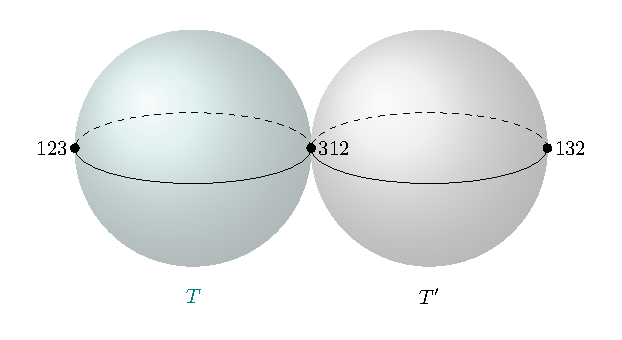
\includegraphics[width=0.75\linewidth]{./fig_springer_fiber.pdf}
        \caption{Springer Fiber $\mathcal{B}_x$}
    \end{figure}
\end{example}

\subsection{Symplectic Duality}

In \cite{braden2016quantizationsconicalsymplecticresolutions}, it is mentioned that the cotangent bundle of flag varieties forms symplectic dual pairs. In particular, we have

\begin{theorem}{\cite{braden2016quantizationsconicalsymplecticresolutions}}
    Let $G$ be a reductive algebraic group and $^LG$ be its Langlands dual. Pick Borel subgroups $B\subset G$ and $^LB\subset{^LG}$. Then $T^*(G/B)$ is symplectic dual to $T^*(^LG/^LB)$. The correspondence of fixed points is given by sending $w$ to $w^{-1}w_\circ$, and the category $\OO$ for $G$ is Koszul dual to that of $^LG$.
\end{theorem}
In particular, $T^*(G/B)$ for type $A$ is self dual.





%Consider the variety $\mathbb{C}^n/S_n$, which consists of all unordered $n$-tuples of complex numbers, alternatively viewed as the orbi-space of the symmetric group $S_n$ acting on $\mathbb{C}^n$ by permuting coordinates.

% For $x\in \mathfrak{sl}_n$, denote by $\CB{x_1, \ldots, x_n}$ the set of eigenvalues of $x$. We have $\sum_{}^{}x_i=\text{tr}\ x=0$.
% This allow us to define the map
% \[
%   \varphi:\mathfrak{sl}_n\rightarrow \CB{(x_1,\dots ,x_n)\mid \sum_{}^{}x_i=0}/S_n\subseteq \mathbb{C}^n/S_n
% \]
% by sending $x$ to the unordered tuple of eigenvalues of $x$.

% \begin{remark}
%   $\mathbb{C}^n/S_n$ is isomorphic to an $n$-dimensional vector space by identifying it with the vector space of complex polynomials in a variable $\lambda$ of degree less than or equal to $n - 1$:
%   $$
%   \psi: \mathbb{C}^{n-1}/S_n \to \mathbb{C}[\lambda]_{(n-1)} \simeq \mathbb{C}^n, \quad (x_1, \ldots, x_n) \mapsto \lambda^n - \prod_{i=1}^n (\lambda - x_i).
%   $$
% \end{remark}

% Define the \vocab{Grothendiect Simultaneous Resolution} of $\mathfrak{sl}_n$ as follows:
% \[
%   \tilde{\mathfrak{sl}}_n=\CB{(x,F)\in \mathfrak{sl}_n \times \mathfrak{B} \mid x \in \mathfrak{b}_F, \textnormal{ i.e. }x(F_i)\subseteq F_i\ \forall\ i}.
% \]
% The extra $F\in \mathfrak{B}$ can be used to order the eigenvalues of $x\in \mathfrak{sl}_n$:
% \[
%   \nu: \tilde{\mathfrak{sl}}_n \rightarrow \CB{(x_1,\dots ,x_n)\mid \sum_{}^{}x_i=0}, (x,F)\mapsto (x_1,\dots ,x_n),
% \]
% where $x_1,\dots ,x_n$ are the eigenvalues of $x$ satisfying $x(F_i/F_{i-1})=x_i(F_i/F_{i-1})$.

% Denote by $\psi:\CB{(x_1,\dots ,x_n)\mid \sum_{}^{}x_i=0}\rightarrow \CB{(x_1,\dots ,x_n)\mid \sum_{}^{}x_i=0}/S_n$ be the order forgetting map, and $\mu: \tilde{\mathfrak{sl}}_n\rightarrow \mathfrak{sl}_n$ be the first projection. We have the following commutative diagram:
% \missing{}

% We define the springer fiber of $x\in \mathfrak{sl}_n$ to be
% \[
%   \mu^{-1}(x)\simeq \mathfrak{B}_x:=\CB{F\in \mathfrak{B}\mid x(F_i)\subseteq F_i}=\CB{B\in \mathfrak{B}\mid x\in \mathfrak{B}}.
% \]

% When $x\in \mathfrak{sl}_n^{sr}$, by definition all eigenvalues are distinct. We have the following lemma:
% \begin{lemma}[lem:]{}
%   For each $x \in \mathfrak{sl}_n^{sr}$, the set $\mathcal{B}_x$ consists of $n!$ distinct flags, and there exists a canonical free action of the symmetric group $S_n$ on $\mathcal{B}_x$, making it a principal homogeneous $S_n$-space.
% \end{lemma}

% \missing{Example of Springer Fiber}

% \subsubsection{Grothendiect's Simultaneous Resolution of \mathintitle{\mathfrak{g}}}

% For general $\mathfrak{g}$, one can define the universal resolution of $\mathfrak{g}$ by
% \[
%   \tilde{\mathfrak{g}} = \{ (x, \mathfrak{b}) \in \mathfrak{g} \times \mathcal{B} \mid x \in \mathfrak{b} \}.
% \]

% Denote by $\mu:\tilde{\mathfrak{g}} \to \mathfrak{g}$ and $\pi:\tilde{\mathfrak{g}} \to \mathcal{B}$ the two coordinate projections of $\tilde{\mathfrak{g}}$.
% For any $\mathfrak{b} \in \mathcal{B}$, the fiber $\pi^{-1}(\mathfrak{b})$ consists of the vector space all elements in $\mathfrak{b}$. Thus, $\pi: \tilde{\mathfrak{g}} \to \mathcal{B}$ is a vector bundle whose fibers are the Borel subalgebras of $\mathfrak{g}$. 

% \begin{proposition}[pps:]{}
%   $\tilde{\mathfrak{g}}$ is a smooth variety with the following $G$-equivariant isomorphism for a fixe $B$:
%   \[
%     G\times _B\mathfrak{b}\xrightarrow[]{\sim}\tilde{\mathfrak{g}}, (g,x)\mapsto (gxg^{-1},g\mathfrak{b}g^{-1}).
%   \]
%   \begin{proof}
%     \missing{}
%   \end{proof}
% \end{proposition}

% $\mu:\tilde{\mathfrak{g}}\rightarrow \mathfrak{g}$ is proper as $\mathfrak{B}$ is compact. Similar as above, define the \vocab{springer fiber} of $x$ in $\mathfrak{g}$ as
% \[
%   \mu^{-1}(x)\simeq \mathfrak{B}_x=\CB{\mathfrak{b}\in \mathfrak{B}\mid x\in \mathfrak{b}}.
% \]

% In two extreme cases, where either $x = 0$ or $x$ is generic, we have

% \begin{itemize}
%   \item If $x = 0$, then $\mu^{-1}(0) = \mathcal{B}$.
%   \item If $x \in \mathfrak{g}^{sr}$, then $\# \mathcal{B}_x = \# W$.
% \end{itemize}
% In fact, we have the following:

% \begin{proposition}[pps:]{}
%   For each $x \in \mathfrak{g}^{sr}$, there exists a canonical free action of $W$ on $\mu^{-1}(x)$, making the projection $\tilde{\mathfrak{g}}^{sr} \to \mathfrak{g}^{sr}$ a principal $W$-bundle.
% \end{proposition}

% Next, we introduce an analogue of the map $v: \mathfrak{g} \to \mathbb{C}^{n-1}$ defined in the case of $\mathfrak{g} = \mathfrak{sl}_n(\mathbb{C})$. This replacement for $\mathbb{C}^{n-1}$ is the abstract Cartan subalgebra $\mathfrak{h}$. For the general case of $\mathfrak{g}$, we define the map:
% $$
% \nu: \tilde{\mathfrak{g}} \to \mathfrak{h}=\mathfrak{b}/[\mathfrak{b}, \mathfrak{b}],
% \qquad 
% (x, \mathfrak{b}) \mapsto x \mod [\mathfrak{b}, \mathfrak{b}].
% $$

% By the Chevalley Restriction Theorem, $\mathbb{C}[\mathfrak{h}]^W\simeq \mathbb{C}[\mathfrak{g}]^G$. Hence we have an embedding $\mathbb{C}[\mathfrak{h}]^W\xrightarrow[]{\simeq }\mathbb{C}[\mathfrak{g}]^G\hookrightarrow \mathbb{C}[\mathfrak{g}]$, inducing a morphism of algebraic varieties
% $\rho:\mathfrak{g}\rightarrow \mathfrak{h}/W$.

% In conclusion, we have the following commutative diagram:
% \missing{}

% \begin{remark}
%   We call $h\in \mathfrak{h}$ \vocab{regular} if it does not belong to any root hyperplanes. Equivalently, the $W$-orbit of $h$ has $\#W$ elements. For another cartan $\mathfrak{h}'$, $h'\in \mathfrak{h}'\subseteq \mathfrak{g}$ is regular if and only if the image of $h'$ in $\mathfrak{h}'\simeq \mathfrak{h}$ is regular in $\mathfrak{h}$. Denote by $\mathfrak{h}^{reg}$ the set of regular elements in $\mathfrak{h}$. Then $\mu^{-1}(\mathfrak{g}^{sr})\simeq \tilde{\mathfrak{g}}^{sr}=\nu^{-1}(\mathfrak{h}^{reg})$.
% \end{remark}

% \subsubsection{Springer Resolution}

% Denote by $\mathfrak{N}$ the nilpotent elements in $\mathfrak{g}$. It is a $\text{Ad}\ G$-stable subvariety of $\mathfrak{g}$. Moreover, it is a cone variety by a $\mathbb{C}^*$ dilation action.
% Recall the map $\mu:\tilde{\mathfrak{g}}\rightarrow \mathfrak{g}$,
% define
% \[
%   \tilde{\mathcal{N}}:=\mu^{-1}(\mathcal{N})=\CB{(x,\mathfrak{b})\in \mathcal{N}\times \mathcal{B}\mid x\in \mathfrak{b}}.
% \]
% Since we have the decomposition $\mathfrak{b}=\mathfrak{h}\oplus\mathfrak{n}$ where $\mathfrak{n}=[\mathfrak{b},\mathfrak{b}]$, $x\in \mathfrak{b}$ is nilpotent if and only if $x\in \mathfrak{n}$.
% Hence the projection $\tilde{\mathcal{N}}\rightarrow \mathcal{B}$ has fiber $\mathfrak{n}$, and 
% \[
%   \tilde{\mathcal{N}}\simeq G\times _B\mathfrak{n}.
% \]

% \missing{pps 3.2.5}

% We can extend the commutative diagram in the previous section as follows:

% \missing{example $T^*\mathbb{P}^1$}

% \begin{theorem}[thm:]{}
%   We have a natural $G$-equivariant Bundle isomorphism
%   \[
%     \tilde{\mathcal{N}}\simeq T^*\mathcal{B}.
%   \]
%   \begin{proof}
%     \missing{}
%   \end{proof}
% \end{theorem}

% \subsubsection{Moment Map and Resolution of Singularity}

% \missing{Hamiltonian action and moment map}
% \begin{corollary}[crl:]{}
%   The projection $\mu:T^*\mathcal{B}=\tilde{\mathcal{N}}\rightarrow \mathcal{N}$ is the moment map with respect to the Hamiltonian $G$-action on $T^*\mathcal{B}$ arising from the $G$-action on $\mathcal{B}$. Furthermore, $\mu$ is surjective and proper.
% \end{corollary}

% $\mu:\tilde{\mathcal{N}}\rightarrow \mathcal{N}$ is called the \vocab{Springer Resolution}.

% \begin{corollary}[crl:]{}
%   $\dim\mathcal{N}=2\dim\ \mathfrak{n}$.
% \end{corollary}

% \begin{corollary}[crl:]{}
%   $\mu^{-1}(\mathcal{N}^{reg})\simeq \tilde{\mathcal{N}}^{reg}$ is an isomorphism. Hence $\mu$ is a resolution of singularities.
% \end{corollary}

